% !TeX spellcheck = it_IT

\chapter{Lavori correlati} \label{chap:related_works}
\section{Segmentazione} \label{sec:segmentazione} 

\begin{figure}[!ht]
  \begin{center}
    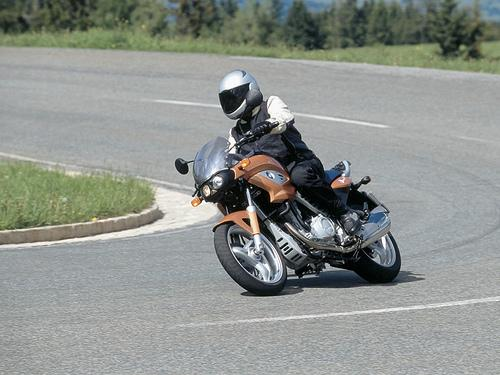
\includegraphics[width=0.4\textwidth]{Immagini/segmantion_example_image.png}
    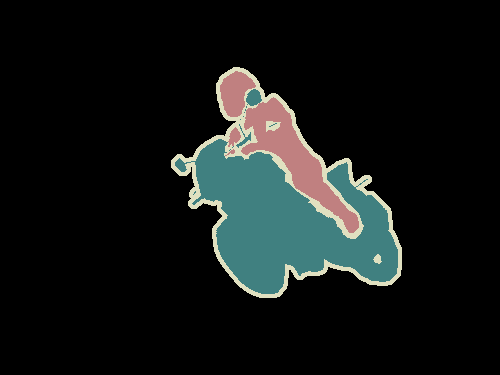
\includegraphics[width=0.4\textwidth]{Immagini/segmantion_example_mask.png}
  \end{center}
  \caption{Segmentazione semantica}
  \label{fig:segmentazione}
\end{figure}

La segmentazione semantica rappresenta un campo di grande interesse e rilevanza
nell'ambito dell'elaborazione delle immagini e della visione artificiale. Questa
tecnica si distingue per la sua capacità d'interpretare il contenuto delle
immagini a un livello semantico, andando oltre la semplice divisione
dell'immagine in regioni omogenee basate su caratteristiche visive come il
colore o la texture. Nello specifico, la segmentazione semantica si prefigge
l'obiettivo di attribuire un'etichetta semantica a ogni singolo pixel
dell'immagine, consentendo così d'identificare e categorizzare le diverse parti
che compongono la scena.  L'obiettivo principale della segmentazione semantica è
quello di fornire una comprensione approfondita del contenuto visivo presente in
un'immagine. Ciò si traduce nella capacità d'identificare e categorizzare
oggetti e regioni, rendendo possibile un'analisi dettagliata e una migliore
interpretazione dei dati visivi.
Un esempio di applicazione della segmentazione semantica la si pu\`o visionare
nella figura \ref{fig:segmentazione}, in questo caso l'obiettivo della segmentazione era quello di 
estrapolare le informazioni relative al motociclista in una classe e le informazioni relative 
al veicolo in un'altra classe, separando entrambe le classi dallo sfondo.



\section{Fully Convolutional Network} 
\begin{figure}[!ht]
  \begin{center}
    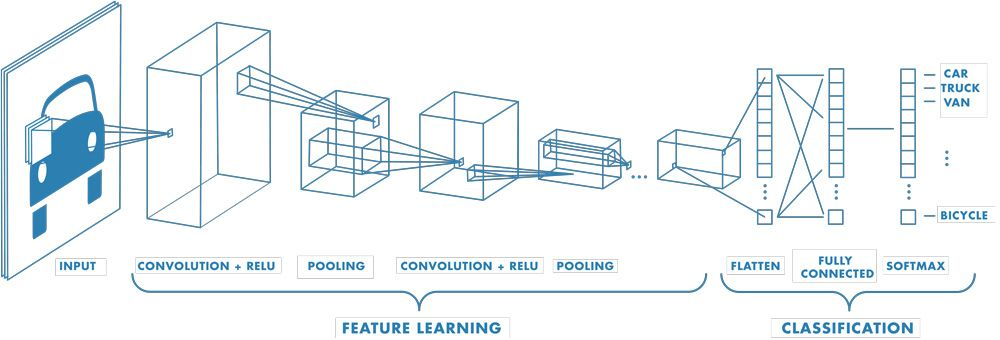
\includegraphics[width=0.8\textwidth]{Immagini/cnn.png}
  \end{center}
  \caption{CNN}
  \label{fig:cnn}
\end{figure}



\label{sec:fcn} L'articolo \textit{Fully
Convolutional Networks for Semantic Segmentation} \cite{long2015fully} propone
l'utilizzo di una tipologia di reti neurali convoluzionali (CNN) che permettono
grazie all'assenza di layer completamente connessi di elaborare immagini di
qualunque dimensione. Questa nuova tipologia di reti migliora notevolmente le capacità di apprendimento delle reti neurali permettendo di produrre mappe
di segmentazione più precise grazie alla loro capacità di apprendimento d'informazioni spaziali.

Le motivazioni riguardanti l'ampio utilizzo nel settore della
\textit{computer vision} sono legate all'assenza di strati completamente
connessi (lineari) che vincolano l'ingresso alla medesima grandezza per ogni
singola immagine, permettendo di fornire in ingresso l'intera immagine e non
frammenti della stessa così da aumentare l'apprendimento spaziale della rete.

Questa maggior flessibilità comporta un addestramento libero da limitazioni
sull'ingresso comportando una maggiore tolleranza agli errori e al rumore
rendendo questa tipologia di reti particolarmente adatte a contesti poveri di
dati.




\section{U-Net} \label{sec:unet} 

\begin{figure}[!ht]
  \begin{center}
    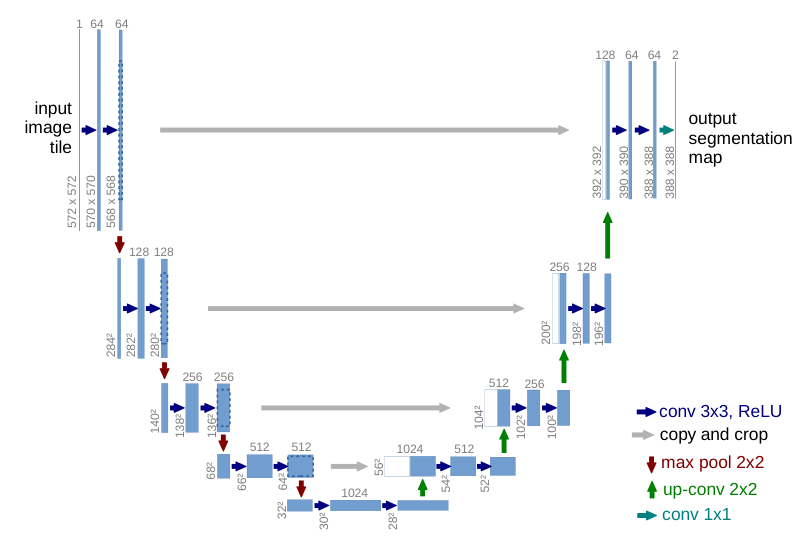
\includegraphics[width=0.8\textwidth]{Immagini/unet.png}
  \end{center}
  \caption{U-Net}\label{fig:unet}
\end{figure}


\subsection{U-Net: Convolutional Networks for Biomedical Image Segmentation}

Nel 2015, Olaf Ronneberger, Philipp Fischer e Thomas Brox hanno introdotto un
nuovo modello di rete neurale convoluzionale chiamato \textit{U-Net} per la
segmentazione semantica d'immagini biomedicali \cite{ronneberger2015unet}.
Questa rete è stata progettata specificamente per affrontare le sfide associate
alla segmentazione d'immagini biomedicali, come la necessità di segmentare
strutture anatomiche precise con un numero limitato d'immagini di
addestramento.

Il modello \textit{U-Net} è caratterizzato da una struttura simmetrica, in cui
la parte "contrattiva" (downsampling) cattura il contesto e la parte "espansiva"
(upsampling) permette una localizzazione precisa. Questa struttura consente alla
rete di combinare le informazioni di contesto con quelle locali, migliorando la
precisione della segmentazione.

Una delle principali innovazioni della \textit{U-Net} è l'introduzione di
collegamenti a salti tra le parti contrattive ed espansive. Questi collegamenti
trasferiscono le caratteristiche spaziali ad alta risoluzione dalla parte
contrattiva a quella espansiva, consentendo una maggiore precisione nella
localizzazione delle strutture segmentate.

Il modello \textit{U-Net} ha dimostrato di ottenere risultati di segmentazione
di alta qualità su diverse applicazioni biomedicali con un numero limitato d'immagini di addestramento, rendendolo uno strumento fondamentale per la
segmentazione semantica in ambito biomedico.




\section{Segmentazione ossea} \label{sec:segmentazione_ossea}

Il lavoro \textit{Towards whole-body CT Bone Segmentation}
\cite{10.1007/978-3-662-56537-7_59} costituisce un'importante analisi volta a
sviluppare metodi e algoritmi avanzati per la segmentazione ossea in immagini
ottenute tramite tomografia computerizzata (TC) di tutto il corpo. Il documento
si concentra sull'importanza della segmentazione ossea nell'ambito medico per
diagnosticare condizioni patologiche e condurre analisi dettagliate del tessuto
osseo.

Il contributo principale dell'articolo consiste nella valutazione di approcci
innovativi e nell'ottimizzazione di tecniche algoritmiche per identificare e
isolare accuratamente le strutture ossee nelle immagini TC. Sottolinea
l'utilizzo di metodologie avanzate di elaborazione delle immagini e
l'applicazione di algoritmi di visione artificiale e machine learning per
ottenere una segmentazione precisa.

L'articolo è rilevante nell'ambito dell'informatica medica in quanto evidenzia
l'applicazione di soluzioni informatiche per l'analisi approfondita delle
immagini mediche, sottolineando l'importanza delle tecniche di segmentazione
ossea per fini clinici e di ricerca biomedica.


\section{Segmentazione di vasi sanguigni}
\label{sec:segmentazione_vasi_sanguigni}

L'articolo \textit{Accurate Retinal Vessel Segmentation via Octave Convolution
Neural Network} \cite{fan2020accurate} propone un approccio innovativo per la
segmentazione precisa dei vasi sanguigni retinici utilizzando le reti neurali a
convoluzione ottava. Questa segmentazione è un'importante fase nell'analisi
delle immagini retiniche in ambito medico.

L'articolo esamina il vantaggio delle reti neurali a convoluzione ottava, un
tipo di rete neurale che sfrutta differenti frequenze spaziali per catturare
dettagli a diverse scale. Questo approccio consente di migliorare la
segmentazione dei vasi sanguigni retinici, consentendo una migliore
comprensione e diagnosi di patologie oculari.

Il lavoro si concentra sull'efficacia delle reti neurali a convoluzione ottava
nel rilevare e isolare i vasi sanguigni della retina, evidenziando come questo
approccio abbia portato a risultati più accurati rispetto a metodi
convenzionali.

In conclusione, l'articolo \textit{Accurate Retinal Vessel Segmentation via
Octave Convolution Neural Network} costituisce un contributo significativo
nell'ambito della segmentazione vascolare retinica, evidenziando l'efficacia
delle reti neurali a convoluzione ottava e la loro importanza nella diagnostica
medica.

